\documentclass[UTF8,adobefonts]{ctexart}

\title{数学思想发展的四个阶段}
\author{郑自强\\
\normalsize
(中国海洋大学,2015级勘察技术与工程) \\[2pt]
学号:15040031045 \\[1.5pt]}
\date{June 24, 2017}

\usepackage{natbib}   %% 使用bibtex做索引文献时需要引入
\usepackage{graphicx}  %% 插入图片时需要引入
\usepackage{epstopdf}  %% 插入eps格式图片,并且使用pdflatex编译时需要引入,用latex编译时不需要引入
\usepackage{CJKutf8}   %% 使用中文目录标题需要引入
\usepackage{lineno}     %% 在伪代码中使用行号时需要引入
\usepackage{indentfirst}  %% 中文首行缩进需要引入
\usepackage[unicode]{hyperref} %%实现交叉引用,目录书签需要引入

\usepackage{amsmath}  %%使用数学公式时需要引入
\usepackage{algorithm}  %%写伪代码时需要引入
\usepackage{algorithmicx}  %%写伪代码需要引入
\usepackage[noend]{algpseudocode}  %%写伪代码需要引入
\usepackage{multirow}      %%表格中需要跨行单元格时需要引入


\newtheorem{theorem}{定理}[section]   %%重定义theorem命令
\newtheorem{lemma}{引理}[section]
\newtheorem{definition}{定义}[section]
\newtheorem{corollary}[theorem]{推论}
\floatname{algorithm}{算法}
\renewcommand{\algorithmicrequire}{\textbf{Input:}}
\renewcommand{\algorithmicensure}{\textbf{Output:}}

\begin{document}
\maketitle      %%生成标题
\pdfbookmark[3]{content}{section.1}   %%生成pdf的书签,3为书签层次,content为书签名,seciton.1为定位点,可以不用。

\begin{abstract}
数学思想是数学的灵魂,是数学不断发展的活力源泉。数学思想是数学活动实践经验的总结和经验的概括,是数学文化的一种传承和不断发展。实践是产生思想方法的源泉,只有在不断的实践中数学才能得到进步和发展。概括和抽象是产生数学思想的关键,数学思想的概括是对自然界一般事物规律的总结和一般化、程序化、模式化的一个过程。数学思想的进步体现在四个方面:(1)渗透于生活;(2)抽象概括;(3)实践巩固;(4)联系发展。\par
\textbf{关键词:} 数学思想,数学文化,联系发展。
\end{abstract}
 
\section{导言}
数学思想是指人们对数学理论和内容的本质的认识,是数学科学发生、发展的根本。数学思想蕴涵在数学知识形成、发展和应用的过程中,是数学知识和方法在更高层次上的抽象与概括而成的数学观点。
\section{正文}
\subsection{渗透生活}
在数学发展史上,有各种各样的数学理论产生、发展、逐渐成熟。一开始一个数学思想的出现可能并不被人门所接受,但它又确确实实起源于生活,并困扰着人们,令人们想要迫切的去解答这一个个难题。我们都知道古时候有结绳记事,人们将具体的事物抽象成数字是有一定的难度的,一头牛被抽象成1,一个苹果也被抽象成1。那么是不是一头牛就等于一个苹果呢?这个问题困扰这我们的祖先,但是这个问题又源于生活,具有其实际的生活意义。后来人们将现实世界的空间形式和具体的数量关系反映到人的意识和更多的专有名次中,数字只是作为一个数量词,而不是具体的实物的代表。显然这样的改变更具有了抽象意义,也更难以理解。不过它大大地方便了人们的生活,让人们不再拘泥于数字和实物之间的一一对应关系。显然我们的数学思想来源于生活,并渗透于生活。\par
新的数学思想的产生往往是社会生活生产中的数学实践和数学研究实践的共同作用。另外数学活动也是数学思想的一种加工的体现。离开了数学活动,数学思想方法就成为脱离实际的抽象的乌托邦,不能用来提高数学信息加工的效率,不能起到发展大脑信息加工机能的作用。因此离开源于具体生活的数学活动,数学思想是没有价值的。那么什么样的活动又可以被称为数学活动呢?我认为数学活动渗透于我们的日常生活中。小至我们牙牙学语时期的数星星活动,大至各种繁琐复杂的数学公式定理推导证明,都可以被称为数学活动,生活离不开数学活动,数学活动又渗透于生活。在不断的数学实践和数学活动中,数学思想能得到最快的发展\cite{黄秦安2001数学文化观念下的数学素质教育}。
\subsection{抽象概括}
抽象概括和推理是数学思维的基本形式,也是数学的基本思想方法\cite{史宁中2011漫谈数学的基本思想}。数学思想方法形成的归纳过程,需要充分的样例积累。用相同的思想方法解决不同形式、不同领域问题的过程经历,是提高归纳的信度,把思想方法一般化、程序化和模式化的基础。最简单的抽象概括就是抽象出变量和变量之间的关系。我们在学习中,经常遇到过解方程的问题,我们解方程的第一步就是抽象出变量,将具体的实物之间的关系转化为数字和变量之间的关系,并把他们用数字符号和逻辑关系表示出来。接下来的一步步才是通过数学原理解方程,这些方程本身是没有任何实际意义的,它们只是我们通过抽象概括得到的。我们不仅需要抽象概括的能力,也需要推理的能力,亚里士多德的三段式推理就是这其中的一个典范,它的过程可以用图~\ref{fig:process}描述。
\begin{figure}
\begin{center}
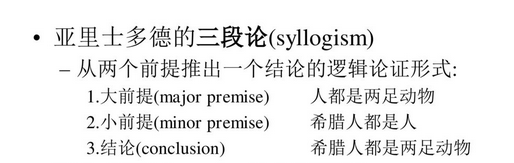
\includegraphics[width=1\linewidth]{data.png}
\hspace{0.05in}
\caption{我们可以看到三段式的核心就是利用两个已经证明出来的结论来推导第三个未知的结论,从这里我们可以看到数学推理的魅力。}
\label{fig:process}
\end{center}
\end{figure}

\subsection{实践巩固}
实践巩固也是数学思想发展的一个必经且十分重要的一个阶段,当新的数学思想产生时,我们怎么才能证明他是行之有效的也具有实际意义?这时候我们就需要实践巩固新的数学思想,数学思想方法是具体问题解决方法的一般化,这种一般化的过程是一种归纳的过程\cite{李大潜2008数学文化与数学教养}。从数学方法的这一根本特性我们可以得出,我们想要检验和巩固新的数学思想,就需要通过实际的数学运算数学实践来支撑。当康托尔发明集合论的时候,许多数学家对于集合论的产生和实际意义报以怀疑的态度,他们并不能接受这种无中生有的集合的思想,这种集合思想是琐碎的,且没有什么具体的意义,被人嗤笑为数字的游戏和逻辑的鬼怪,所以他们对康托尔的这个集合概念并不能很深入的理解。\par
但是当集合论在高等数学和更加完备的数学体系中大放异彩的时候,集合论重建了整个数学体系和系统,它将许多琐碎繁杂的定理变得更加简单,并支撑起了整个数学体系。由此我们可以发现一个新的数学理论思想的出现是需要很多理论基础进行支撑的,没有一个完备的系统作为其支柱,数学体系是很容易崩塌的。无独有偶,当集合论的不完备性被罗素发现时,整个数学体系再一次崩塌,引发了第三次数学危机,为了解决第三次数学危机,数学家们又提出了有穷集合和无穷集合的概念,目前第三次数学危机还尚未解决。从这个不断提出数学思想,不断实践,不断完善的过程中,我们可以得到实践巩固是数学思想发展的一个重要环节。
\subsection{联系发展}
最后我们需要认识到的是数学思想现在是和其他学科联系发展的,它并不仅仅只局限于数学领域,它同许多新兴学科共同发展,在同其他学科的交流联系中数学思想得到了不断发展\cite{才翰2006数学教育心理学}。拿最近新兴的机器学习为例,机器学习的理论基础就是数学原理和数学思想,它起源于数学,但是它在发展的过程中又推动了数学思想的发展。由于它更偏重与实际应用,所以它旨在解决一些实际问题,它在发展的过程中促进了很多数学方面的发展,比如生成对抗网络,卷积神经网络,递归神经网络等等。这些算法的兴起都依赖于数学思想的进步,另一方面,当这些算法风靡时,它又带给了我们更多的思考,我么从后验的角度去总结它为什么生效,哪些工作能加快其的发展。在不断的总结和完善的过程中,一些基础学科又得到发展。所以数学思想和方法是联系发展的,它是和其他学科共同发展,而不是完全独立的一门科学。通过抽象,把外部世界与数学有关的东西抽象到数学内部,形成数学研究的对象,构建了数学与外部世界的桥梁。
\section{结论}
数学思想就是在这四个过程的不断交叠的过程中得到不断发展,并具有了极强的生命力支撑其不断发展。


\bibliographystyle{plain}
\bibliography{reference}  %%插入索引文献
\end{document}
